\documentclass{sig-alternate}

\begin{document}
%
% --- Author Metadata here ---
\conferenceinfo{18-697}{Fall '14 Pittsburgh, PA USA}
\CopyrightYear{2014}
% --- End of Author Metadata ---

\title{Clustering for Controlling Stochastic Optimization using Feedback}
\subtitle{Applied to Newspaper Article Title Category Prediction}

\numberofauthors{2} 
\author{
\alignauthor
Kevin Brennan\\
       \affaddr{Carnegie Mellon University}\\
       \affaddr{5000 Forbes Avenue}\\
       \affaddr{Pittsburgh, PA}\\
       \email{kbrennan@andrew.cmu.edu}
% 2nd. author
\alignauthor
Gavriel Adler\\
       \affaddr{Carnegie Mellon University}\\
       \affaddr{5000 Forbes Avenue}\\
       \affaddr{Pittsburgh, PA}\\
       \email{gya@andrew.cmu.edu}\\
}


\maketitle
\begin{abstract}
In this paper, we develop a method that uses a feedback controller in order to control the desired number
of local optima.
\end{abstract}

%%@Kevin-->Not sure what these are
% A category with the (minimum) three required fields
%\category{H.4}{Information Systems Applications}{Miscellaneous} %I commented out this line
%A category including the fourth, optional field follows...
%\category{D.2.8}{Software Engineering}{Metrics}[complexity measures, performance measures] %I commented out this line

\terms{Classification, Feedback, Stochastic Optimization} %I put some down...

\keywords{Controlled Clustering, Naive Bayes, KMeans, Title Category Classification} %I put some down...

\section{Introduction}
In optimization problems there are often multiple local optima. In order to reduce the complexity of the solution space


\section{Related Research}
Background

\section{Method}
\begin{figure*}[t]
\centering
\fbox{
  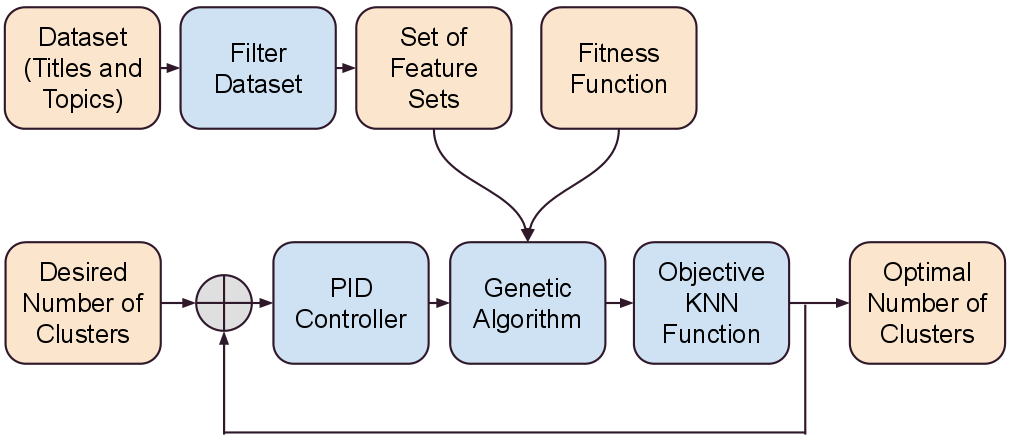
\includegraphics[width=0.8\textwidth]{pipeline.png}}
\caption{The Algorithm Pipeline}
\label{fig:pipeline}
\end{figure*}
\subsection{Pipeline Overview}
Our pipeline, as seen in Figure~\ref{fig:pipeline}, consists of a few independent pieces put together in a control loop. To initialize the pipeline, we first separated the titles into a training and a testing set. We then made a list of words that appear in the titles of the training set and filtered the data set into our feature sets, or sets of bags of words from that list. In the control loop, we get our error value from the difference between the optimal number of clusters returned by the objective K-Means function and the desired number of clusters. The error and the PID controller created a $\phi$ term representing exploration vs. exploitation. We generated sets of bags of words from the training set list and passed each into the genetic algorithm along with the $\phi$ term, and each returned a locally optimal bag of words. These optimal bags were clustered to find the optimal number of clusters, and the loop restarts. Each section of the algorithm is discussed in detail below.

\subsection{Genetic Algorithm}
\begin{figure}[t]
\centering
\fbox{\rule{0pt}{2in}
  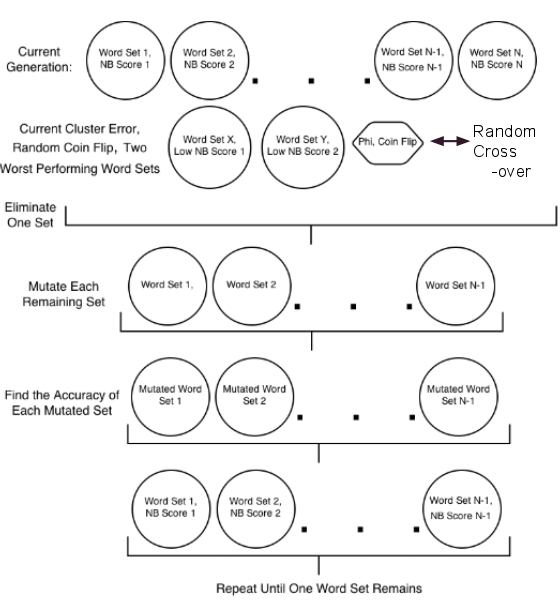
\includegraphics[width=0.5\textwidth]{genetic_algo.png}}
\caption{The flow of one iteration of the genetic algorithm}
\label{fig:genetic_algo}
\end{figure}
Our genetic algorithm operated on a set of bags of words, and converged to a single locally optimal bag of words. At each round of the genetic algorithm, the Naive Bayes score on the testing set was calculated for each bag of words. The lowest two scores competed for survival, and the victor was based on both the $\phi$ exploration/exploitation term and a random coin flip. After one bag was killed, each remaining bag was mutated and additional randomized cross-over between trials was added in to further diversity. Our solution set was created by running several trials of the genetic algorithm on many randomly generated sets of bags of words.\\
\indent In the mutation step, the algorithm attempted to replace each word in the bag of words with a new word taken from the titles in the training set. If the Naive Bayes score of the bag of words with the new word was higher than it was with the old word, the new word replaced the old word, otherwise the new word was discarded.\\
\indent In our genetic algorithm, we did not follow CITEPAPERHERE and user Hamiltonian Distance in the clustering algorithm, instead we decided to try something different and creative and used Naive Bayes results. We passed the number of true positives, true negatives, false positives, and false negatives to the clustering algorithm, hoping this would create diverse results with some bags of words strong in each case. In the end we found this approach did not fare well and the results converged to a single cluster very quickly, and therefore would recommend not using our process but Hamiltonian Distance in the future.

\subsection{Clustering Algorithm}
Our clustering algorithm operates based on the Objective K Nearest Neighbor function. For this algorithm, we use a variable number of nodes to group the 
solution set from the genetic algorithm trials into clusters. For each number of nodes, we cluster the data using K-Means to 

\subsection{Implementation}

\subsection{Controller}

\section{Results}

\section{Conclusions}

\section{Future Work}

\section{Acknowledgments}

\cite{salas:calculus}

%
% The following two commands are all you need in the
% initial runs of your .tex file to
% produce the bibliography for the citations in your paper.
\bibliographystyle{abbrv}
\bibliography{sigproc}  % sigproc.bib is the name of the Bibliography in this case

\end{document}
